\lhead{\emph{Arquitectura}}
\chapter{Arquitectura}

Sumada a las herramientas creadas en el sistema, es necesario llevar a cabo una serie de operaciones que posibiliten el acceso a servicios más básicos tales como la autenticación de los usuarios del sistema, %TODO etc

Con el objetivo de mejorar la situación actual en la infraestructura a analizar, se tratan los siguientes problemas.

\section{Autenticación de los usuarios}

Los usuarios del sistema deben ser capaces de acceder al sistema mediante un sistema de credenciales que posibilite el uso de cualquier nodo del sistema con el mismo conjunto de claves. Dicho enfoque es el propio de la infraestructura actual del sistema, que en concreto sigue un enfoque centralizado.

Un primer intento de posibilitar la ``universalización'' del acceso ha sido la creación de los mismos usuarios en cada uno de los nodos, utilizando el mismo par usuario-contraseña en cada uno de ellos. Sin embargo, este enfoque impide una escalabilidad sencilla y requiere un mantenimiento continuo (suponiendo que se añaden usuarios periódicamente). Por ello únicamente las pruebas iniciales de las plataformas que requieren acceso a la funcionalidad de autenticación han sido realizadas siguiendo este enfoque, pero siempre desacoplando al máximo el sistema de acceso del resto de la lógica del programa, con el objetivo de facilitar su reemplazo.

Habiendo descartado dicha estrategia, queda como alternativa más adecuada a las necesidades del sistema el uso de la infraestructura presente en el centro académico.

La infraestructura del centro comprende varios servicios que interactúan entre sí, siendo el pilar clave el servidor LDAP (\textit{Lightweight Directory Access Protocol})\citationneeded. Dicho servidor almacena la información de todos los usuarios de la infraestructura y da acceso a cualquier equipo de varias de las aulas de la Facultad.
\begin{figure}[H]
	\centering
	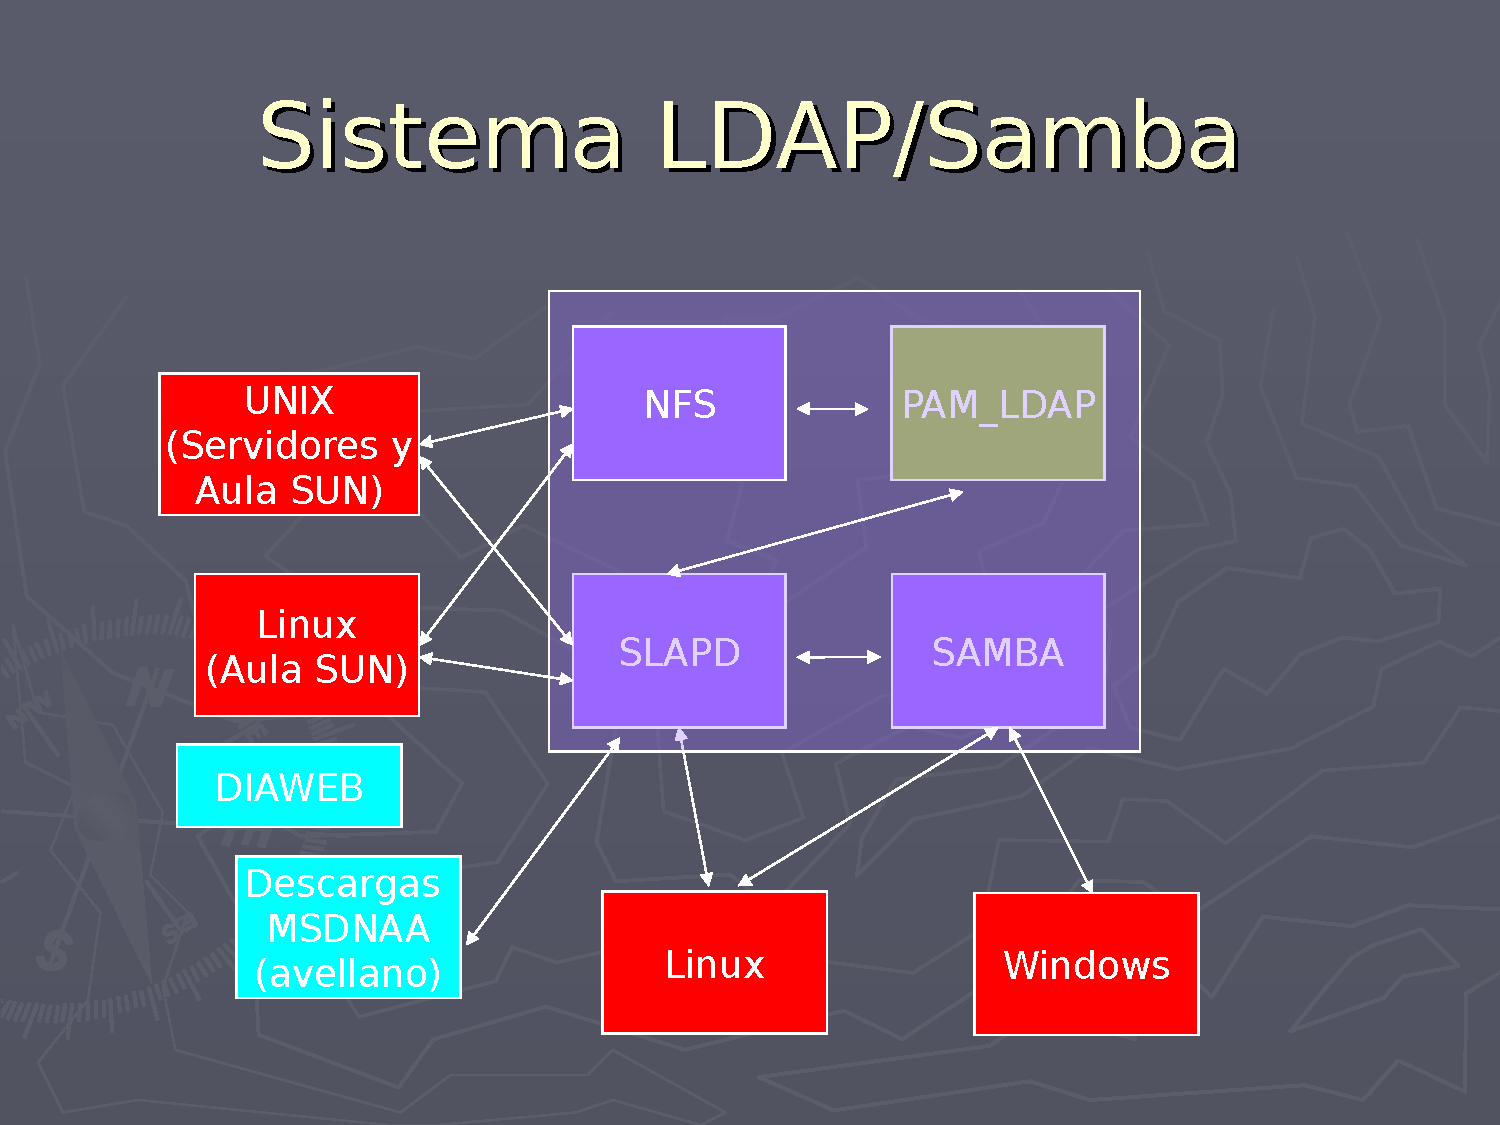
\includegraphics[width=0.7\textwidth]{Chapter4/Figures/LDAP.pdf}
	\caption{Esquema de los diferentes componentes del sistema de autenticación y gestión de archivos, así como de una serie de componentes adicionales. Obsérvese la interacción entre los componentes situados en el rectángulo interior}
	\label{fig:arquitectura_ldap}
\end{figure}

\subsection{Características en detalle}

Debido a la heterogeneidad de los diferentes equipos presentes en la infraestructura, el sistema debe posibilitar el acceso a todos los equipos utilizando el mismo conjunto de credenciales. Esto implica que el sistema debe ser compatible con al menos los sistemas operativos GNU/Linux, Microsoft Windows y Solaris. Por ello se interconecta el servidor LDAP con Samba, así como el PAM (\textit{Pluggable Authentication Module}) tanto en el cliente como el servidor.

Sin embargo el sistema permite también que los usuarios puedan almacenar información en un espacio centralizado al que es posible acceder desde cualquier equipo, facilitando la copia de ficheros entre nodos, uniformidad de los diferentes equipos. Esto se consigue utilizando un servidor NFS (\textit{Network File Storage}).

\subsection{Utilización en el sistema}

En el sistema se aprovechará principalmente la funcionalidad de autenticación provista por el servidor LDAP, debido a que uno de los objetivos principales del sistema es evitar ``cuellos de botella'' debido al uso de un servidor de almacenamiento central. Herramientas como el \textbf{deployer} facilitarán la replicación de servicios en su lugar. En cualquier caso, se plantea permitir el acceso al NFS desde el sistema como complemento, pero no como espacio principal de almacenamiento.

El sistema aprovecha el módulo PAM para realizar el proceso de autenticación.

\section{Compilación}

Si bien el sistema Raspberry Pi es capaz de compilar el \textit{software} que después utilizará, en ocasiones es beneficioso delegar dicha tarea a otro componente que realice el proceso por el nodo en cuestión y posteriormente añadir los archivos ejecutables al sistema. Este enfoque reduce el tiempo de trabajo de forma significativa, como observaremos posteriormente.%proporcione los resultados al solicitante.

\subsection{Creación de un compilador cruzado}

Un compilador cruzado (\textit{cross-compiler})es una herramienta capaz de generar código para una architectura utilizando un equipo con otra arquitectura diferente.%TODO: http://en.wikipedia.org/wiki/Cross_compiler
El uso de compiladores cruzados 